\chapter{Monte Carlo simulation}
In the current thesis, all the Monte Carlo simulations were performed by using Geant4.9.5.p01 toolkit\cite{Agostinelli:2003fg}. The purposes of the Monte Carlo simulations were to produce dummy data with specific processes and to evaluate all the detector effects, such as energy losses of particles, multiple scatterings, the detector acceptance, and the tracking performance with the chamber position resolution.

We employed pre-implemented physics list QGSP\_BERT to produce neutron spectrum, where all the neutrons passing through the NC were detected even without energy deposit and later scaled by the NC efficiency of 23\% in the analysis procedure. Other detector efficiencies were also 100\% in the data generation and were taken into account when compared to the real experimental data. The detector hit positions and timings were smeared with their resolutions. For the neutron missing-mass analysis, a true value of the generated missing mass was smeared by the missing-mass resolution in Fig.\ref{fig-mmresol} after the event selection. The event selection was done by the same procedure as the real-data analysis, except for upstream part of the beam analysis.

\section{Geometry implementation}
Precise implementation of the detector and other material geometries are essential for this kind of simulations. We implemented all detectors downstream of the D5 magnet with calibrated positions by the beam data. Thin materials such as black sheets and aluminized Mylar sheets used for wrapping scintillators, and chamber wires were ignored. Support structures for the detectors were also not implemented. For materials around the target, we implemented the target cell, the radiation shield and the CFRP vacuum vessel and its aluminum cap. We did not implemented the He transfer pipe and most of the cooling part of the cryogenic system. Note that materials implemented for the Monte Carlo simulation were exactly same including their positions as those considered in the energy loss calculation of the particles.
\section{Event generator}
We constructed an event generator which could generate an event with final state particles defined in an input parameter file. The reaction vertex position of an event was generated according to the measured kaon beam distributions of the position and direction. The $z$ position was randomly selected and only vertices within the fiducial volume were accepted. A positive kaon was generated as a kaon beam at the vertex point toward upstream of the beam line with a realistic momentum distribution and was forbidden to decay. 

\subsection{Treatment of the Fermi motion}
For the kinematical distribution of the final state particles, the Fermi motion of the nucleon in $^3$He were considered, while the cross section was the fixed values. First, we generated all the final state particles including the spectator(s) uniformly in the $n$ body phase space. Then, the spectators, if existed, were fed into the momentum filters at Laboratory system, to be consistent with the measured fermi momentum distribution in $^3$He in the $(e,e'p)$ reaction\cite{Jans:1982aw}.  The density distribution of the spectator momenta were described by the double Gaussian distribution as shown in Fig. \ref{fig-geantfermi}. 

\begin{figure}[]
\begin{center}
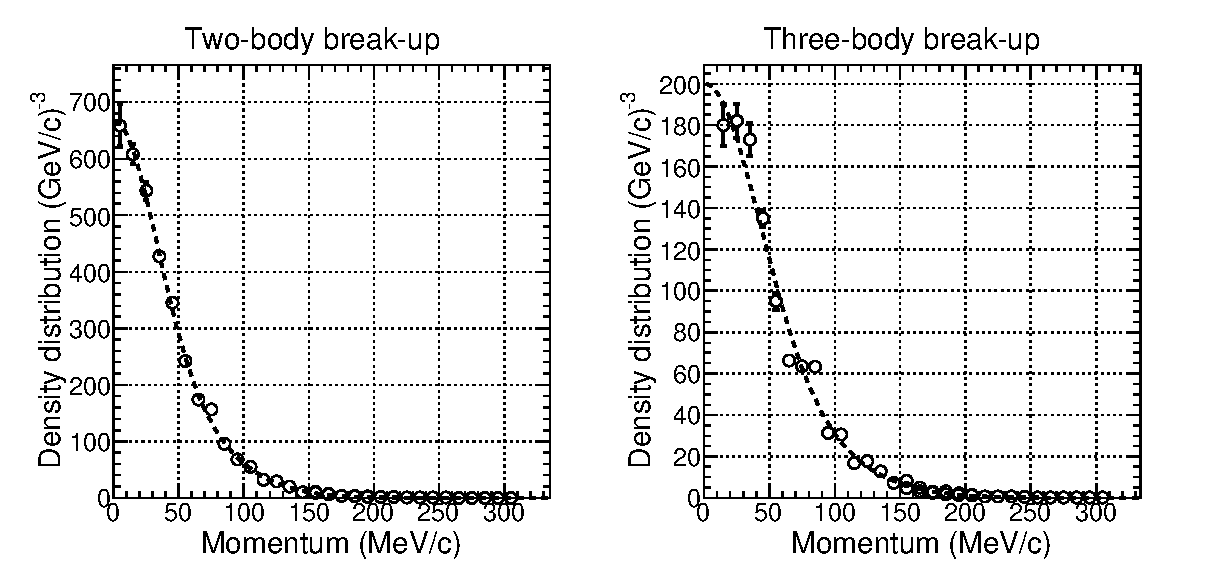
\includegraphics[width=\columnwidth]{./fig/fermi.eps}
\caption[Momentum density distributions of spectators in $^3$He.]{Momentum density distributions of spectators in $^3$He used in the Monte Carlo simulations. If we have one spectator particle ( deuteron or a nucleon in the two nucleon process) the two-body break-up data was used (left), while the distribution (right) was used for the events with two spectator particles.}
\label{fig-geantfermi}
\end{center}
\end{figure}  

\subsection{Angular distribution}
We also considered the angular distribution of the final state particles if the reaction had two body final state (except for the spectator(s)) and there was measured angular distribution. The filter of the angular distribution was applied in the CM frame of the two final-state-particle system with generated momentum described above.

\subsection{Generated elementary processes}
The simulated spectrum in Fig. \ref{fig-sim1n} was generated with known elementary processes listed in Table \ref{tab-kpreaction} and Table \ref{tab-knreaction}. The relative strength of each process were determined by the measured cross sections at around 1 GeV/$c$. Cross sections for some processes were extrapolated from the data with lower/higher beam momentum.  We simply considered $^3$He as 2 protons and 1 neutron, the total cross section of $K^-$-$^3$He ($\sigma_{K^{-3}{\rm He}}$) was assumed to be
\begin{eqnarray*}
\sigma_{K^{-3}{\rm He}} &=& 2\times \sigma_{K^-p} + \sigma_{K^-n},
\end{eqnarray*}
where $\sigma_{K^-p}$ and $\sigma_{K^-n}$ are the total cross sections of $K^-p$ and $K^-n$ elementally processes, respectively. The spectator was assumed to be always a deuteron in the $K^-p$ processes, while two protons had fermi motions independently in the $K^-n$ processes.
\begin{table}[]
\caption[$K^-p$ elementary processes implemented in the Monte Carlo simulation.]{$K^-p$ elementary processes implemented in the Monte Carlo simulation. A sign of inequality in a kaon beam momentum ($p_{lab}$) shows we got the cross section at 1 GeV/$c$ by an extrapolation. The data used for the extrapolation is in CERN-HERA-83-02.}
\begin{center}
\begin{tabular}{l|ccccc} 
\hline\hline				
Final state	&	$p_{lab}$	&	CS	&	error	&	Ref.	&	Production			\\
	&	GeV/$c$	&	(mb)	&	(mb)	&		&	angle			\\
\hline													
$K^-p$ (elastic)	&	1.005	&	21.75	&	0.73	&	\cite{Conforto:1976iu}	&	\cite{Conforto:1976iu}			\\
\hline													
$\Lambda\pi^+\pi^0\pi^-$	&	1.001	&	0.41	&	0.04	&	\cite{Anonymous:G7Qq9mMJ}	&	-		\\
$\Lambda\pi^+\pi^-$	&	1.001	&	4.66	&	0.22	&	\cite{Anonymous:G7Qq9mMJ}	&	-		\\
$\Lambda\pi^0$	&	1.001	&	3.40	&	0.20	&	\cite{Anonymous:G7Qq9mMJ}	&	\cite{Anonymous:G7Qq9mMJ}		\\
$\Lambda2\pi^0$	&	$>$0.86	&	1.00	&	1.00	&		&	-		\\
$\Lambda\eta$	&	1.001	&	0.22	&	0.07	&	\cite{Anonymous:G7Qq9mMJ}	&	\cite{Rader:1973dl}	(1.021 GeV/$c$)	\\
$\Lambda\rho^0$	&	$<$1.138	&	0.10	&	0.10	&		&	x		\\
$\Lambda(1405)\pi^0$	&	$>$0.85,$<$1.138	&	0.40	&	0.40	&		&	x		\\
$\Lambda(1520)\pi^0$	&	1.005	&	2.44	&	0.17	&	\cite{Cameron:1977kn}	&	\cite{Cameron:1977kn}		\\
$\Sigma^+\pi^+2\pi^-$	&	1.001	&	0.05	&	0.01	&	\cite{Anonymous:G7Qq9mMJ}	&	-		\\
$\Sigma^+\pi^0\pi^-$	&	1.001	&	1.04	&	0.08	&	\cite{Anonymous:G7Qq9mMJ}	&	-		\\
$\Sigma^+\pi^-$	&	1.001	&	1.95	&	0.11	&	\cite{Anonymous:G7Qq9mMJ}	&	\cite{Anonymous:G7Qq9mMJ}		\\
$\Sigma^0\pi^+\pi^0\pi^-$	&	1.001	&	0.18	&	0.03	&	\cite{Anonymous:G7Qq9mMJ}	&	-		\\
$\Sigma^0\pi^+\pi^-$	&	1.001	&	0.53	&	0.05	&	\cite{Anonymous:G7Qq9mMJ}	&	-		\\
$\Sigma^0\pi^0$	&	1.005	&	0.92	&	0.12	&	\cite{Conforto:1976iu}	&	\cite{Baxter:1973ed}	(0.934 GeV/$c$)	\\
$\Sigma^02\pi^0$	&	$>$0.86	&	0.50	&	0.50	&		&	-		\\
$\Sigma^-\pi^+$	&	1.001	&	1.53	&	0.09	&	\cite{Anonymous:G7Qq9mMJ}	&	\cite{Anonymous:G7Qq9mMJ}		\\
$\Sigma^-\pi^+\pi^0$	&	1.001	&	0.90	&	0.08	&	\cite{Anonymous:G7Qq9mMJ}	&	-		\\
$\Sigma^-\pi^+2\pi^0$	&	$<$1.15	&	0.10	&	0.10	&		&	-		\\
$\Sigma^-2\pi^+\pi^-$	&	1.001	&	0.01	&	0.01	&	\cite{Anonymous:G7Qq9mMJ}	&	-		\\
$\Sigma(1385)^+\pi^-$	&	1.005	&	1.12	&	0.12	&	\cite{Cameron:1978et}	&	\cite{Cameron:1978et}		\\
$\Sigma(1385)^0\pi^0$	&	$<$1.263	&	0.00	&	0.00	&		&	x		\\
$\Sigma(1385)^-\pi^+$	&	1.005	&	1.99	&	0.19	&	\cite{Cameron:1978et}	&	\cite{Cameron:1978et}		\\
$p\pi^+\pi^-K^-$	&	$<$1.138	&	0.02	&	0.02	&		&	-		\\
$p\pi^0K^-$	&	1.005	&	0.97	&	0.05	&	\cite{Cameron:1977kn}	&	-		\\
$p\pi^-K^0$	&	1.001	&	0.51	&	0.07	&	\cite{Anonymous:G7Qq9mMJ}	&	-		\\
$pK^{*-}$	&	1.005	&	0.26	&	0.03	&	\cite{Cameron:1978ih}	&	\cite{Cameron:1978ih}		\\
$n\pi^+\pi^-K^0$	&	$<$1.161	&	0.01	&	0.01	&		&	-		\\
$n\pi^+K^-$	&	1.005	&	0.63	&	0.04	&	\cite{Cameron:1978ih}	&	-		\\
$n\pi^0K^0$	&	$>$0.85,$<$1.15	&	0.80	&	0.80	&		&	-		\\
$nK^0$	&	1.000	&	6.45	&	0.04	&	\cite{AlstonGarnjost:1977ec}	&	\cite{Anonymous:G7Qq9mMJ}	(1.001 GeV/$c$)	\\
$nK^{*0}$	&	1.005	&	0.20	&	0.02	&	\cite{Cameron:1978ih}	&	\cite{Cameron:1978ih}		\\
$\Delta^+K^-$	&	1.005	&	0.35	&	0.03	&	\cite{Cameron:1977kn}	&	x		\\
$\Delta^0K^0$	&	1.005	&	0.73	&	0.07	&	\cite{Cameron:1978ih}	&	x		\\
inelastic total	&		&	34.39	&	1.52	&		&				\\
\hline													
Total	&		&	56.14	&	1.69	&		&				\\
\hline\hline												
\end{tabular}
\end{center}
\label{tab-kpreaction}
\end{table}%

\begin{table}[]
\caption[$K^-n$ elementary processes implemented in the Monte Carlo simulation.]{$K^-n$ elementary processes implemented in the Monte Carlo simulation. A sign of inequality in a kaon beam momentum ($p_{lab}$) shows we got the cross section at 1 GeV/$c$ by an extrapolation. The data used for the extrapolation is in CERN-HERA-83-02.}
\begin{center}
\begin{tabular}{l|ccccc} 
\hline\hline				
Final state	&	$p_{lab}$	&	CS	&	error	&	Ref.	&	Production		\\
	&	GeV/$c$	&	(mb)	&	(mb)	&		&	angle		\\
\hline												
$K^-n$ (elastic)	&	0.963	&	20	&	1	&	\cite{Armenteros:1970fo}	&	\cite{Damerell:1977wj}	(0.935GeV/$c$)	\\
\hline												
$\Lambda\pi^+2\pi^-$	&	0.963	&	0.26	&	0.06	&	\cite{Armenteros:1970fo}	&	-		\\
$\Lambda\pi^0\pi^-$	&	0.995	&	3.79	&	0.42	&	\cite{Corden:1977ba}	&	-		\\
$\Lambda\pi^-$	&	0.995	&	4.8	&	0.34	&	\cite{Corden:1977ba}	&	\cite{Cox:1970gq}	(1.189 GeV/$c$)	\\
$\Lambda(1405)\pi^-$	&	$<$1.45	&	0.1	&	0.1	&		&	x		\\
$\Lambda(1520)\pi^-$	&	$<$1.45	&	0.5	&	0.5	&		&	x		\\
$\Sigma^+\pi^02\pi^-$	&	0.963	&	0.03	&	0.02	&	\cite{Armenteros:1970fo}	&	-		\\
$\Sigma^+2\pi^-$	&	0.995	&	1.18	&	0.12	&	\cite{Corden:1977ba}	&	-		\\
$\Sigma^0\pi^0\pi^-$	&	$>$0.854	&	0.5	&	0.5	&		&	-		\\
$\Sigma^0\pi^-$	&	0.995	&	1.35	&	0.18	&	\cite{Corden:1977ba}	&	\cite{Hepp:1976ix}	(($\Sigma\pi)^-$, 0.854GeV/$c$)	\\
$\Sigma^-\pi^+\pi^0\pi^-$	&	0.963	&	0.24	&	0.04	&	\cite{Armenteros:1970fo}	&	-		\\
$\Sigma^-\pi^+\pi^-$	&	0.995	&	0.69	&	0.09	&	\cite{Corden:1977ba}	&	-		\\
$\Sigma^-\pi^0$	&	0.995	&	0.89	&	0.13	&	\cite{Corden:1977ba}	&	\cite{Hepp:1976ix}	(($\Sigma\pi)^-$, 0.854GeV/$c$)	\\
$\Sigma^-2\pi^0$	&	$>$0.854	&	0.3	&	0.3	&		&	-		\\
$\Sigma(1385)^0\pi^-$	&	$<$1.45	&	0.5	&	0.5	&		&	x		\\
$\Sigma(1385)^-\pi^0$	&	$<$1.45	&	0.5	&	0.5	&		&	x		\\
$p\pi^-K^-$	&	0.995	&	0.95	&	0.1	&	\cite{Corden:1977ba}	&	-		\\
$n\pi^-K^0$	&	0.995	&	1.49	&	0.23	&	\cite{Corden:1977ba}	&	-		\\
$nK^{*-}$	&	$<$1.45	&	0.2	&	0.2	&		&	x		\\
$\Delta^0K^-$	&	$<$1.45	&	0.05	&	0.05	&		&	x		\\
$\Delta^-K^0$	&	$<$1.45	&	1	&	1	&		&	x		\\
inelastic total	&		&	19.32	&	1.60	&		&			\\
\hline												
Total	&		&	39.32	&	1.89	&		&			\\
\hline\hline												
\end{tabular}
\end{center}
\label{tab-knreaction}
\end{table}%

\section{Response of the NC}
There is little experimental information on nuclear reactions of neutrons with the momenta of around 1 GeV/$c$, corresponding to the kinetic energies of several hundred MeV. Although the neutron detection efficiency of the NC was evaluated from the data by using the quasi-free charge-exchange reaction as described in Sec. 3.8.5, here we shows the calculated efficiency by the simulation based on Geant4 QGSP\_BERT\_ HP package as a reference. In the simulation, we also set a "online" threshold of 0.5 MeV for the energy deposit on a NC segment.

\subsection{Momentum dependence of the NC detection efficiency\label{sec-geantnc}}
Figure. \ref{fig-ncsimeff}(left) shows the calculated efficiency for the various offline thresholds as a function of the momentum. In the simulation, the detection efficiency is almost flat around the interest region of 1.2$\sim$1.4 GeV/$c$ and down to $\sim$0.6 GeV/$c$. Therefore, we ignored the momentum dependence in the current analysis.

\subsection{Energy deposit distribution}
Figure \ref{fig-ncsimeff}(right) shows a comparison of the relative efficiency at the quasi-free peak ($\sim$1.15 GeV/$c$) between the simulation and the data, where the data points are scaled to be consistent with the simulation at 8 MeV$ee$. The threshold dependence is well reproduced by the simulation. It means that the energy deposit distribution of the simulation is reliable.

\begin{figure}[]
\begin{center}
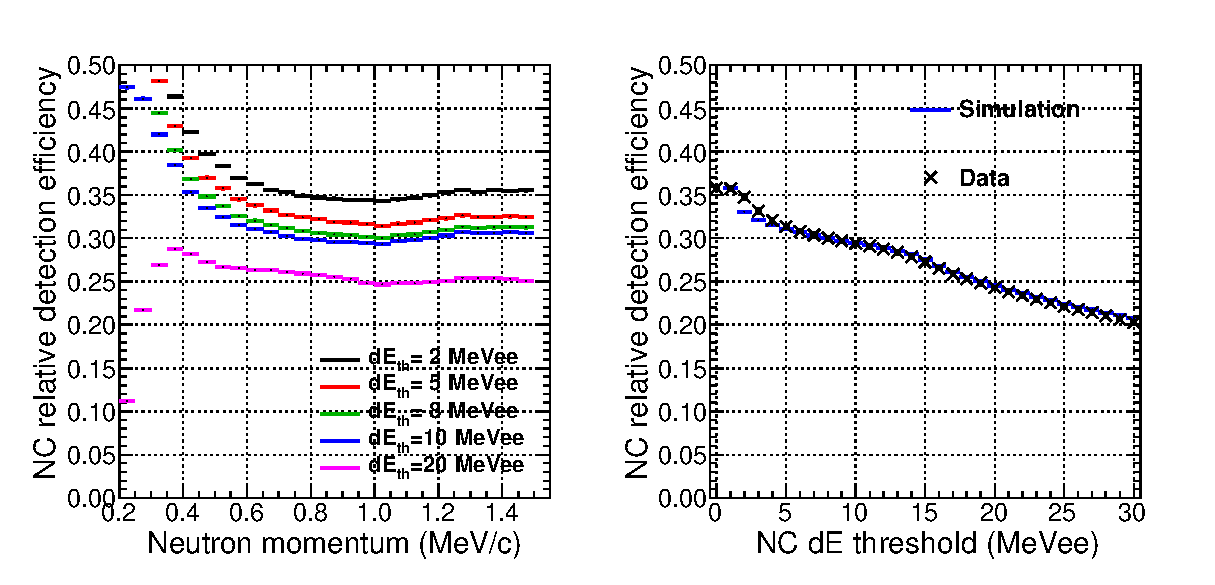
\includegraphics[width=\columnwidth]{./fig/nc-simeff.eps}
\caption[Simulated NC responses.]{(left) Momentum dependence of the NC relative efficiency obtained by the Monte Carlo simulation. (right) Comparison of the NC relative detection efficiency at the quasi-free peak ($\sim$1.15 GeV/$c$) between the data and the simulation. The data points are the yields around the quasi-free peak, which are scaled to be consistent with the simulation at 8 MeV$ee$.}
\label{fig-ncsimeff}
\end{center}
\end{figure}  

